
\cleardoublepage

\chapter{Background}
\label{background}

This chapter begins with a brief summary of existing research that involves automated plant mapping.  The main differences between these solutions and the proposed mapping system are highlighted.  Next, the various coordinate systems used throughout the mapping process are defined, as well as the background theory on converting between camera pixels and world coordinates.  This conversion and it's underlying assumptions are at the core of the image-based mapping system. 

\section{Similar Research}
\label{section:similar_research}

There are two different approaches to precision plant mapping.  One is to create the map during the planting process, that is as the plants or seeds are being deposited into the ground.  The other is to determine the plant locations after the planting is finished.  This section presents an existing solution to the former approach and then discusses different methods for determining plant locations after they've been planted in the ground. 

\subsection{Planter Based Solutions}

The research described in ~\citep{Sun:2010} evaluated two different methods for mapping tomato transplants during the planting process.  The first was the use of an encoder attached to the planting wheel in order to sense when a plant should be ejected from the planter. This wheel encoder had an angular resolution that corresponded to a ground resolution of 0.45 millimeters.  There was naturally displacement between when the plant was released from the planter and where it actually ended up in the field due to the forward velocity of the planter.  This displacement was experimentally calculated on a small set of plants and then accounted for during the mapping.  

The second method was to use an infrared optical beam-splitter to detect when the stem of a plant passed through the beam.  As shown in Figure~\ref{figure:tomato_planter}, the beam-splitter was placed roughly 1 meter behind the planting wheel in order to give the plant time to settle once the soil has been pressed down around it.  

\begin{figure}
	\centering
    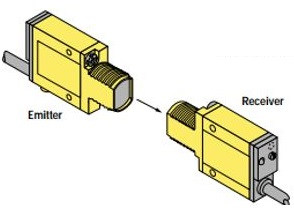
\includegraphics[height=1.5in]{figures/tomator_optical_sensor.jpg}
    \caption[Infrared beam-splitter]{Infrared optical sensors setup in beam-splitting configuration. Adapted from~\citep{Sun:2010}}
    \label{figure:optical_sensor}
\end{figure}

The mapping platform consisted of a Holland model 1600 planter equipped with a centimeter level \ac{rtk} system using a single antenna.  In order to determine the planter heading, a \ac{sse} linear regression algorithm was used on three consecutive position measurements. To further increase the accuracy of the system, a dual axis inclinometer was used to take into account the non-zero roll and pitch angles of the planter.  This sensor, along with the \ac{rtk} receiver, encoder, and beam-splitter, were all connected to a National Instruments cRIO embedded computer with a \ac{fpga} for parallel data logging.    

\begin{figure}
	\centering
    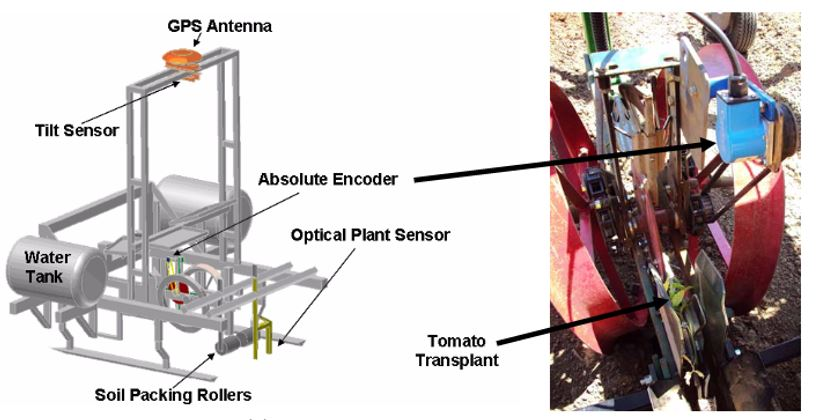
\includegraphics[width=6in]{figures/tomator_planter.jpg}
    \caption[Tomato mapping platform]{Schematic diagram of planter showing sensor placement. Adapted from~\citep{Sun:2010}}
    \label{figure:tomato_planter}
\end{figure}

In an experiment with 512 tomato plants, the beam-splitting sensor detected 491 objects, however only 249 of those corresponded to actual plants.  The rest were due to soil clods or other debris.  Many of the actual plants were missed due to being bent or planted at an angle and thus too low to pass through the beam.  Unsurprisingly, these results were considered to be very poor and were attributed to the difficulty in finding a good height for the beam-splitter to be placed above the ground.

The second method, the encoder wheel, detected 527 planting events.  The additional 15 events were due to plants not being placed in the planter wheel by the operator.  After the offset calibration mentioned above, both the encoder wheel and beam-splitter sensor achieved average mapping accuracies of approximately 3 centimeters in the east direction and 1 centimeter in the north direction.  The movement of the planter was primarily in the east direction which explains the larger errors.  The results of the experiment are copied in Table~\ref{table:tomato_results}.  

\begin{table}
    \begin{center}
    \caption[Tomato mapping results]{Tomato mapping results.}
    \begin{tabular}[c]{|c|c|c|}
        \hline
        Measurement & Infrared Sensor & Encoder Wheel \\
        \hline
        Mean Error - East (cm)   & 3.7       &  3.0    \\
        Mean Error - North (cm)  & 1.2       & 1.0     \\
        Std. Dev. - East (cm)    & 2.1       & 1.6     \\
        Std. Dev. - North (cm)   & 0.9       & 0.8     \\
        \hline
    \end{tabular}
    \label{table:tomato_results}
   \end{center}
\end{table} 
          
While the encoder wheel was effective in creating an accurate plant map, this approach has several drawbacks. One of these drawbacks is it requires close monitoring of the sensors' status. If an issue goes unnoticed then it could potentially result in a large section of the map being unusable, without a straightforward way to redo the mapping. Another disadvantage is it's difficult to extend this method to include differentiating between different groups of plants, which for the experiment described in this thesis was considered a requirement.
          
It's also worth noting that both ~\citep{Nørremark:2007} and ~\citep{Ehsani:2004} implemented similar systems using infrared seed detectors, and these sensors were much more successful at reliably determining plant locations than the beam-splitting method described above.  The accuracy results of these systems were similar to those shown in Table~\ref{table:tomato_results}.
          
\subsection{Post-Planting Solutions}

Many different methods in the past have been investigated for locating plants in the field.  While this is an essential step in creating a field map for a post-planting solution, this area of research mainly focuses on using this information in real-time as opposed to the creation of a map.  For example, in a tilling application the system would locate the plants as the platform is driving through the field rather than relying on a pre-existing map of plant locations.  As a result, the research typically focuses on the effectiveness of finding plants instead of the accuracy of their coordinates.  

These methods of locating plants primarily involve non-contact sensors such as cameras or depth sensors.  For example, ~\citep{Andujar:2013} used the distance and reflectance values from a \ac{lidar} type sensor to effectively differentiate between green plants and soil. ~\citep{Kise:2005} successfully used a stereo vision camera to map rows of soy bean plants based on estimated height measurements from a three-dimensional reconstruction.  In addition, ~\citep{Panneton:2014} investigated combining color and near-infrared spectrum along with three-dimensional plant data to improve the robustness of locating plants.  ~\citep{Soille:2000} used a watershed algorithm with morphological operators to extract a pre-known characteristic such as vein structure.  This is especially useful in situations where plants and weeds are overlapping, and it's not easy to differentiate between them.

Each of these methods have their advantages, but it was determined that a solution based on monocular, color vision is preferred for the proposed mapping system.  This is because plant height information is not useful right after transplanting, and single image solutions are inherently simpler and less expensive. 

\section{Coordinate Systems}

A key step in any mapping process is the correct choice of coordinate systems.  In the context of mapping, coordinates define the location of an item in the field with respect to a reference point.  These coordinate systems, or frames of reference, are typically fixed to items that are significant in the mapping process, which include the Earth, field, platform, and cameras.  The specific coordinate systems used in this research are discussed in the following sections.

\subsection{Latitude and Longitude}

A commonly used frame that is fixed to the Earth is a spherical coordinate system with the angles referred to as latitude and longitude. However, since the Earth is not a sphere these angles are projected onto an ellipsoid, called a datum.  The datum that is used in this research is the \ac{wgs}, which is the default datum used by the \acf{gps}. ~\citep{datums:2016}  The third dimension is altitude and is measured relative to the surface of the ellipsoid.  Coordinates in the frame are denoted $(\Phi, \lambda, A)$.

\begin{figure}
	\centering
    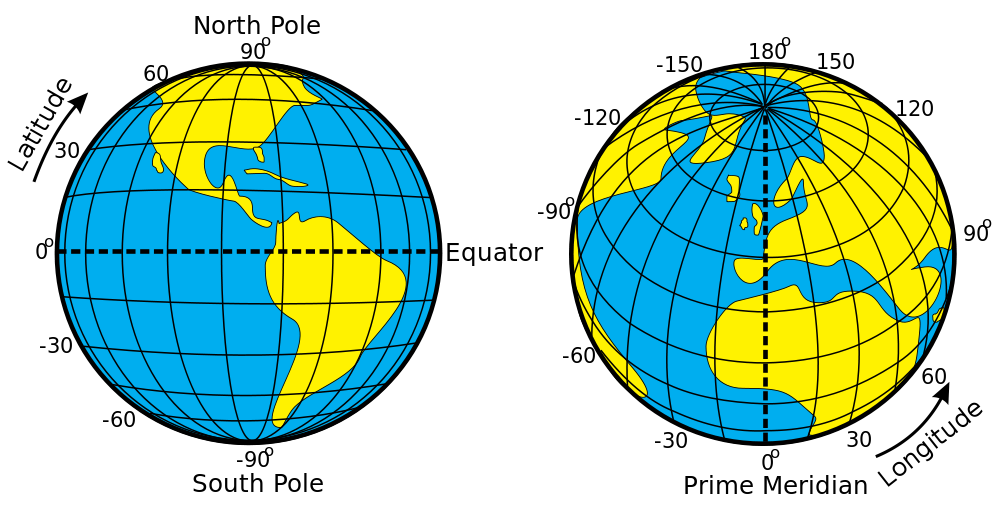
\includegraphics[height=2.5in]{figures/latitudelongitude.png}
    \caption[Latitude and longitude]{Illustration of Latitude $(\Phi)$ and Longitude $(\lambda)$. Obtained under the Creative Commons License from the Wikimedia Commons.}
\end{figure}

\subsection{Universal Transverse Mercator (UTM)}
\label{section:utm}

In order to describe points on the Earth's surface in a two-dimension plane, a projection model must be used on the latitude and longitude coordinates.  The projection model used in this research is the \acf{utm} which splits the Earth into 60 lateral bands, examples of which are shown in Figure~\ref{utm_zones}.  In each zone an item is described by its easting, northing and altitude coordinates.  However, due to how the platform coordinate system is defined it's beneficial to have the Z axis in the downward direction.  This requires the easting and northing be switched to maintain a right-handed coordinate system. Therefore, \acf{utm} coordinates are described by $(N,E,D)$.  Another important modification is that the Z, or down, component is measured relative to the ground rather than the \ac{wgs} ellipsoid. 

\begin{figure}
	\centering
    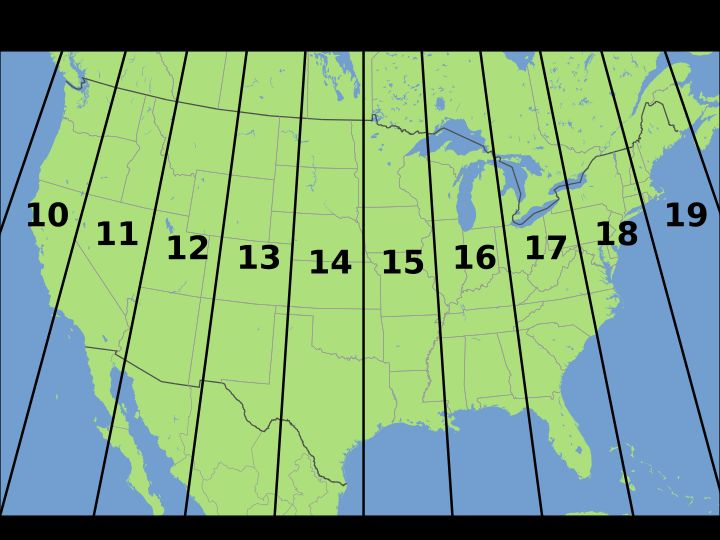
\includegraphics[height=2.5in]{figures/utm_zones.jpg}
    \caption[UTM zones]{Visualization of UTM zones over the United States. Obtained under the Creative Commons License from the Wikimedia Commons.}
    \label{utm_zones}
\end{figure}

\subsection{Field Coordinate System}
\label{section:field_coordinates}

One issue with the northing and easting described by \ac{utm} is that rows in a fields are not always planted north and south or east and west.  Many of the post-processing steps benefit from removing this relative field orientation. A new field coordinate system is defined where the y-axis runs parallel to the rows and increases in the planting direction of the first row, and the x-axis increases in the direction of increasing row numbers.  The origin is selected so that all items in the field have positive x and y coordinates.   Similar to \ac{utm}, the units of this frame are meters.  Coordinates in this frame are denoted $(x_f,y_f,z_f)$.

\begin{figure}
	\centering
    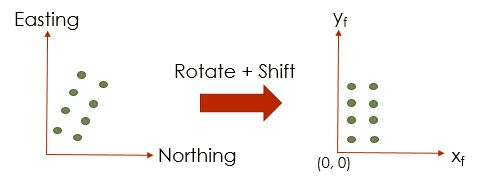
\includegraphics[height=2in]{figures/field_coordinates_small.jpg}
    \caption[Field coordinates]{Conversion from modified \ac{utm} coordinate frame (left) to field coordinate frame (right).}
    \label{field_coordinates}
\end{figure}

\subsection{Platform Coordinate System}
\label{platform_coordinate_system}

Another useful coordinate system is one fixed to the platform holding the cameras.  This coordinate system allows the relative spacing and orientation between the cameras and the \ac{gnss} antenna to be specified.  In addition, this coordinate system defines how the platform's orientation is defined in terms of Euler angles, which is useful for accounting for non-level camera orientation.  The axes of this coordinate system are displayed in Figure~\ref{platform_frame} which defines the x-axis out of the front of the platform, the y-axis out the right hand side and the z-axis orthogonal in the downward direction.  

\begin{figure}
	\centering
    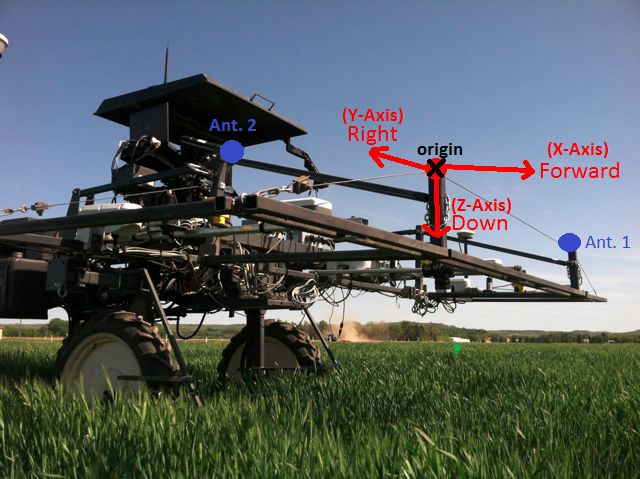
\includegraphics[height=4in]{figures/platform_frame_2_gps.jpg}
    \caption[Platform coordinate frame]{Example of the platform coordinate frame on a tractor system with two \ac{gnss} antennas shown in blue. The origin is the average of these antenna locations and is shown as a black X.}
    \label{platform_frame}
\end{figure}

\subsection{Camera Coordinate System}

The camera coordinate system describes the location of objects in the world relative to the camera body.  Typically, a camera coordinate system is defined by the x-axis out of the right hand side of the camera, the y-axis out of the bottom and the z-axis along the optical axis.  For this application, however, an alternative camera coordinate system is defined which has the x-axis out of the top of camera, the y-axis out of the right side and the z-axis along the optical axis.  This definition is used so that when the camera is mounted on the platform facing the ground with the top forward, the camera axes will align with the forward-right-down platform coordinate system.  This makes the meaning of the standard roll-pitch-yaw Euler angles consistent and is also enforced by the data collection program.  The origin is defined to be located at a distance $f$ in front of the imaging sensor along the optical axis, where $f$ is the focal length of the lens.  This is discussed more in the following section.

\begin{figure}
	\centering
    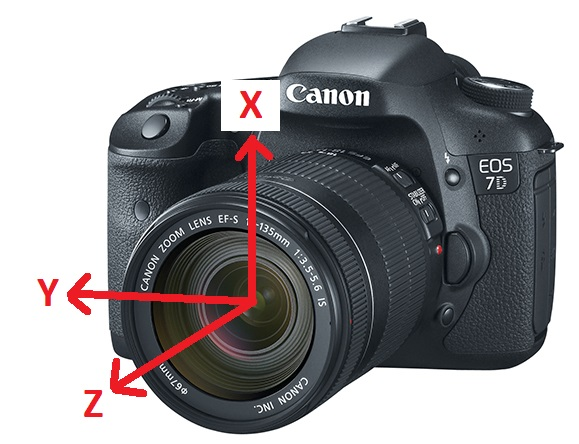
\includegraphics[height=2.5in]{figures/camera_frame_canon.jpg}
    \caption[Camera coordinate frame]{Image showing camera coordinate axes.}
    \label{figure:camera_axes}
\end{figure}

\section{Coordinate Projections}
 
 An important step when post-processing the images is converting between pixel and world coordinates, which is also the subject of many computer vision algorithms.  Since pixels are described in $\mathbb{R}^2$ and world points in $\mathbb{R}^3$, this conversion requires a projection.  
 
 However, before this conversion can be defined a model must be chosen which describes how points in the world are projected onto the imaging sensor.  This section first presents the model used in this research and then discusses two equivalent methods that can be used for converting coordinates.  
 
 \subsection{Projection Model}
 
 A common choice for a thin, convex lens is the central perspective imaging model shown in Figure~\ref{projection_model} ~\citep{Coorke:2013}. This model is based on the concept of an ideal lens that is treated as an equivalent pin-hole.  This implies the lens is perfectly focused and has no geometrical distortions.  The ideal lens will have two focal points along the optical axis as can be seen in Figure~\ref{focal_points}.  The central perspective model defines the image plane to be at the focal point in front of the lens, which is the left focal point shown in the figure.  
 
 \begin{figure}
 	\centering
     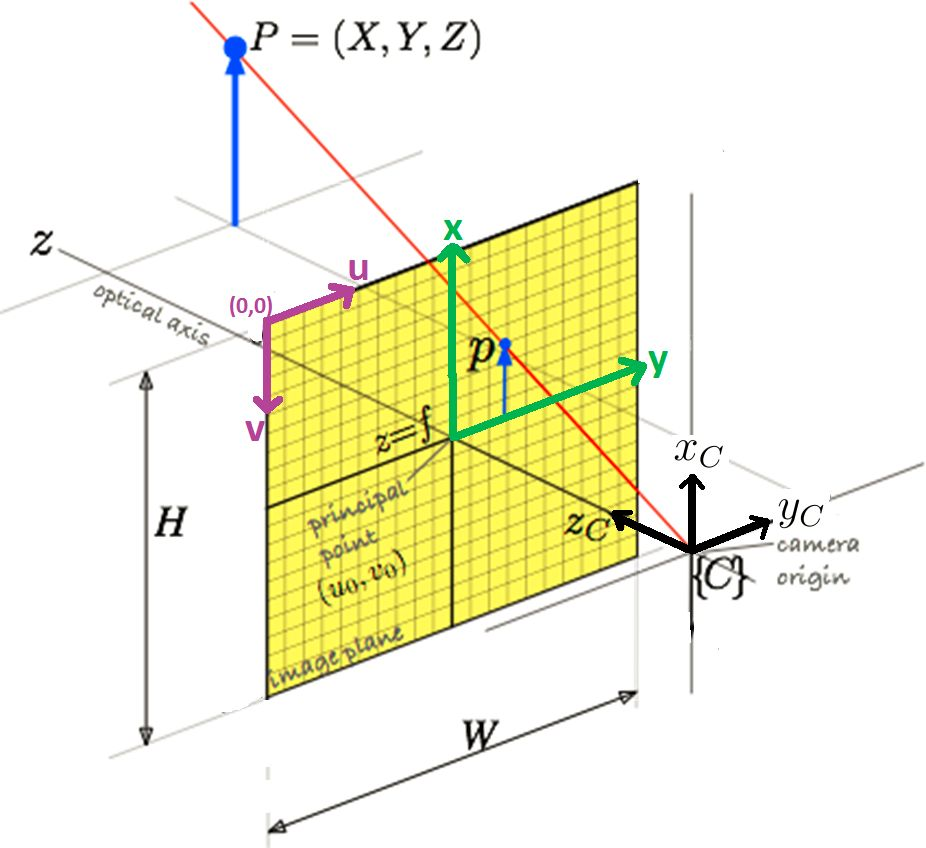
\includegraphics[height=4.5in]{figures/projection_model.jpg}
     \caption[Projection model]{Central perspective imaging model showing the image plane in yellow.  Adapted from "Robotics, Vision and Control" 1st edition, by Peter Coorke, 2013, p.252. Modified to show pixel frame in purple, the sensor frame in green, and switched the ordering of the camera axes.}
     \label{projection_model}
 \end{figure}

\begin{figure}
	\centering
    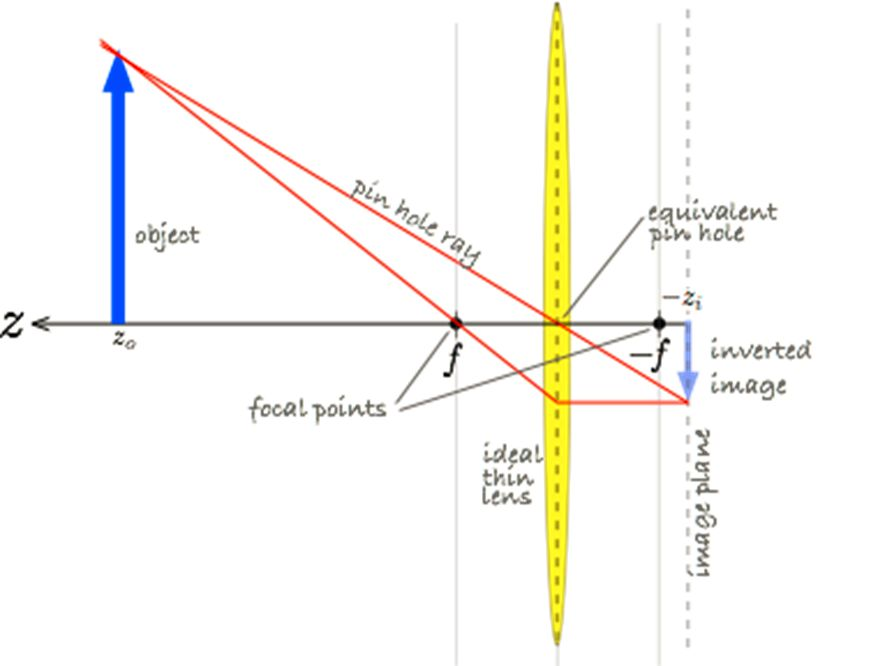
\includegraphics[height=2.5in]{figures/projections_two_focal.jpg}
    \caption[Focal points]{Equivalent pin-hole lens showing both focal points. Adapted from "Robotics, Vision and Control" 1st edition, by Peter Coorke, 2013, p.252}
    \label{focal_points}
\end{figure} 

 Points in the image plane can be described using two different coordinate frames.  The first is the sensor frame and the second is the pixel frame.  The origin of the sensor frame is located at the point where the optical axis intersects the image plane.  A point in this frame is described by $(x,y)$, where the axes are in the same direction as the camera frame and are shown in blue in Figure~\ref{projection_model}.  
 
 On the other hand, the origin of the pixel frame is located at the top left corner of the image plane, and the x-axis increases to the right and the y-axis downwards.  A pixel's location is denoted as $(u,v)$ rather than $(x,y)$.  The center of the image sensor is referred to as the principal point and is denoted $(u_0,v_0)$. Another key difference between these frames is the units.  The sensor frame has units of millimeters while the pixel frame has units of pixels.

 \subsection{Projection Methods}

 The conversion between pixel and world coordinates can go both ways, and both are used in the post-processing pipeline.  However, going from pixel to world coordinates is used more often and is slightly more challenging. That is what is presented in this section. The conversion involves three frame transformations   
\begin{center}
 Pixel $(u,v)$ $\rightarrow$ Sensor $(x,y)$ $\rightarrow$ Camera $(X,Y,Z)$ $\rightarrow$ World $(N,E,D)$
\end{center}
 
 This is referred to as a backwards projection since it is projecting two-dimensional points out into the world.  As mentioned above, this is more challenging because depth information is lost during the forward projection as the image is captured.  Sometimes, multiple cameras or images are used to recover this depth information.  Although in this application the height of objects being mapped are relatively small.  For that reason, an assumption is made that every point in the world frame has a height of zero.  This reduces the world to a plane and results in a $\mathbb{R}^2$ to $\mathbb{R}^2$ mapping which is possible with a single image. 
 
 There are two different methods for performing this backwards projection. The first method discussed operates in Euclidean space and is more intuitive to understand.  The second method builds on this first method by instead working in Projective space.  This produces a more efficient, but equivalent, conversion.  Both of these methods use the central perspective model, and both make the same assumptions about the camera and lens.  These are:
 \begin{itemize}
 \item The lens does not cause any distortion. 
 \item There is no skew or displacement in how the image sensor is positioned within the camera.
 \item The focal length exactly matches the manufacturer's specification.
 \end{itemize}

 All of these assumptions are false to some extent. However, it is possible to correct them using certain camera calibration procedures ~\citep{Zhang:1999}. For the system presented in this research, however, these effects are considered negligible. 
 
 \subsubsection{Euclidean Space}
 
 The first transformation in the projection sequence is to convert pixel coordinates to sensor coordinates.  Using the frame definitions shown in Figure~\ref{projection_model}, this can be represented in matrix form as 
 
\[
\begin{bmatrix} x \\ y \end{bmatrix}
=
\begin{bmatrix} 
 0 & -\rho_h \\
 \rho_w & 0 
\end{bmatrix}
\begin{bmatrix} u \\ v \end{bmatrix}
+
\begin{bmatrix} \rho_h v_0 \\ \rho_w u_0 \end{bmatrix}
\]
 where $\rho_w$ and $\rho_h$ are the width and height of each pixel in millimeters, and $u_0$ and $v_0$ are the coordinates of the principal point in pixels.   The next transformation is to convert from sensor coordinates to camera coordinates.  It's clear from the projection model that if the sensor coordinates are combined with the focal length $f$ as
 \begin{center}
 $(x,y,f)$
 \end{center}
 then the result is a directional vector in the camera frame, but with units of millimeters rather than meters. The last frame transformation is to describe this vector in terms of the world frame.  This can be accomplished by a rotation matrix $R$
 \begin{equation}
 \label{rotation_eq}
 \begin{bmatrix} n \\ e \\ d \end{bmatrix}
 =
 R *
 \begin{bmatrix} x \\ y \\ f \end{bmatrix}
 \end{equation}
 where this rotation matrix is composed from the active, extrinsic rotations about the world's north, east and down axes in that order, by angles $\phi$ (roll), $\theta$ (pitch), and $\psi$ (yaw).  These are the Tait-Bryan angles of the camera frame with respect to the world frame.  Technically, this is a passive rotation by negative angles since the vector is changing between bases, but using active rotations avoids many double negatives.
  \begin{align}
  \label{rotation_equation}
  R &= R_z(\psi)*R_y(\theta)*R_x(\phi) \\ \notag
    &= \begin{bmatrix} \cos(\psi)  & -\sin(\psi) & 0 \\ 
                        \sin(\psi) & \cos(\psi) & 0 \\
                         0         &   0         & 1  \end{bmatrix} 
       \begin{bmatrix} \cos(\theta) & 0 & \sin(\theta) \\ 
                             0      & 1 &       0        \\
                      -\sin(\theta) & 0 & cos(\theta) \end{bmatrix}
       \begin{bmatrix} \ 1 &    0       & 0           \\ 
                         0 & \cos(\phi) & -\sin(\phi) \\
                         0 & \sin(\phi) & cos(\phi)  \end{bmatrix} \\ \notag
    &= \begin{bmatrix} \cos(\theta)\cos(\psi) & \sin(\phi)\sin(\theta)\cos(\psi) - \cos(\phi)\sin(\psi) &  \sin(\phi)\sin(\psi) +  \cos(\phi)\sin(\theta)\cos(\psi) \\
    \cos(\theta)\sin(\psi) & \cos(\phi)\cos(\psi) + \sin(\phi)\sin(\theta)\sin(\psi) &  \cos(\phi)\sin(\theta)\sin(\psi) - \sin(\phi)\cos(\psi) \\
     -\sin(\theta) & \sin(\phi)\cos(\theta) & \cos(\phi)\cos(\theta)     \end{bmatrix}
  \end{align}
  
 Lowercase coordinates $(n,e,d)$ in equation \ref{rotation_eq} are used to designate that these components are in the north, east, and down directions, but the units are still in millimeters meaning this does not represent the world point yet.  The position of this vector in the world frame is given by the camera's world position

 \begin{equation}
 \label{translation_equation}
 T = 
 \begin{bmatrix} T_x \\ T_y \\ T_z \end{bmatrix} =
 \begin{bmatrix} N_{cam} \\ E_{cam} \\ D_{cam} \end{bmatrix}
 .
 \end{equation}

 The actual world point can be found by calculating the intersection of this vector, $(n,e,d)$, with the flat plane of the Earth given by the equation $D=0$.  This can be done by parameterizing the vector as a line with parameter $S$ as 
 
 \begin{equation}
 \label{parameter_ned}
 \begin{bmatrix} N \\ E \\ D \end{bmatrix} =
 S \begin{bmatrix} n \\ e \\ d \end{bmatrix}
 + T
 ,
 \end{equation}
 plugging in the third component, $D$, into the plane equation and solving for
 \begin{center}
 $S = -T_z / d$
 , 
 \end{center}
 which can be plugged back into equation \ref{parameter_ned}.  If $d$ is zero then the position vector is parallel to the Earth's surface and will never intersect it.   

 While this method is easy to visualize, it requires multiple steps for each pixel that must be converted to world coordinates.  A more efficient method is presented in the next section.

 \subsubsection{Projective Space}
 \label{section:projection_space}
 
 An ideal solution would be to describe the backwards projection from the pixel plane to the world plane as a single matrix that can be applied in one step.  In order to do this, coordinates in each frame must be converted into the Projective space which adds an extra coordinate.  This coordinate represents scale, and a set of coordinates in this space is referred to as homogeneous coordinates.  There are many benefits of using homogeneous coordinates, including
 \begin{enumerate}
 \item performing translations and rotations in a single matrix.
 \item avoiding unnecessary division in intermediate calculations, which is typically slower than other operations.
 \item representing a coordinate at infinity with real numbers.
 \end{enumerate}
 
 Homogeneous coordinates are followed by an apostrophe in order to differentiate them from regular Euclidean coordinates.  For example, in the pixel frame coordinates can be described in Projective space as $(u',v',w')$ where 
 \begin{center}
 $u' = u*w'$ and $v'=v*w'$
 .
 \end{center}
 
 In a backwards projection the pixel coordinates $(u,v)$ are what is known, so $w'$ is always set to 1.  This is so it does not change the overall scale.  In order to convert from pixel to sensor coordinates, the same relationship using the pixel sizes and principal point are used. However, when homogeneous coordinates are substituted this relationship can be described as a single matrix.
 
 \[
 \begin{bmatrix} x' \\ y' \\ z' \end{bmatrix}
 =
 \begin{bmatrix} 
     0   & -\rho_h & \rho_h v_0 \\ 
  \rho_w &    0    & \rho_w u_0 \\
     0   &    0    &      1  
 \end{bmatrix}
 \begin{bmatrix} u' \\ v' \\ 1 \end{bmatrix}
 \]
 
 This is typically referred to as the inverse parameter matrix, or $K^{-1}$.  The second transformation is to convert sensor coordinates to camera coordinates.  A consequence of defining the origin of the camera frame to be the location of the equivalent pin-hole is that all incoming rays of light converge to the origin of the frame.  This leads to the simple relationship using the focal length $f$ of
  
  \begin{center}
  $x=fX/Z$  and $y=fY/Z$
  ,
  \end{center}
  which can easily be derived by similar triangles.  When described as homogeneous coordinates this relationship becomes 
  
  \begin{center}
  $x'=fX$, $y'=fY$, and $z'=Z$
  \end{center}
  or in matrix form as
   \[
   \begin{bmatrix} X_u \\ Y_u \\ Z_u \end{bmatrix}
   =
   \begin{bmatrix} 
       1/f &   0   &  0 \\ 
       0   &  1/f  &  0 \\
       0   &   0   &  1  
   \end{bmatrix}
   \begin{bmatrix} x' \\ y' \\ z' \end{bmatrix}
   .
   \]
  
  The subscript $u$ denotes that these coordinates in the camera frame are unscaled, similar to how $(x,y,f)$ is not correctly scaled in the Euclidean method.  Also note that $(X_u, Y_u, Z_u)$ are not homogeneous coordinates.  This matrix is referred to as the inverse camera matrix, or $C^{-1}$. 
  
  The last frame transformation is to go from the camera to world frame and correctly scale the position vector.  This can be done in one step if homogeneous world coordinates $(N',E',D',S')$ are used.  In terms of the rotation matrix $R$ and camera translation vector $T$ defined in equations \ref{rotation_equation} and \ref{translation_equation}  
     \[
     \begin{bmatrix} R^{-1} & -T \end{bmatrix}
     \begin{bmatrix} N' \\ E' \\ D' \\ S' \end{bmatrix}
     =
     \begin{bmatrix} X_u \\ Y_u \\ Z_u \end{bmatrix}
     .
     \]
     
 If each element in $R$ is denoted by its row, $i$, and column, $j$, as $R_{ij}$, and since the inverse of an orthogonal matrix is equal to its transpose, then this is expanded to
 
      \[
      \begin{bmatrix} r_{11} & r_{21} & r_{31} & -T_x \\
                      r_{12} & r_{22} & r_{32} & -T_y \\
                      r_{13} & r_{23} & r_{33} & -T_z \\
      \end{bmatrix}
      \begin{bmatrix} N' \\ E' \\ D' \\ S' \end{bmatrix}
      =
      \begin{bmatrix} X_u \\ Y_u \\ Z_u \end{bmatrix}
      .
      \]
      
  This matrix is clearly not invertible and the assumption that $D=0$ must be enforced.  Since $D'=D/S'$ then $D'$ is also zero, and it can be removed along with the third column of the matrix.   After the matrix is inverted this results in 
  
  \[
    \tilde{p} =
    \begin{bmatrix} N' \\ E' \\ S' \end{bmatrix}
      = 
    \begin{bmatrix} r_{11} & r_{21} & -T_x \\
                    r_{12} & r_{22} & -T_y \\
                    r_{13} & r_{23} & -T_z \\
    \end{bmatrix}^{-1}
    \begin{bmatrix} X_u \\ Y_u \\ Z_u \end{bmatrix}
  .
  \]
 
  Even though an entire column of the rotation matrix is discarded, no information is lost as this column can be described as the cross product of the first and second columns.  This inverted matrix is denoted $\xi^{-1}$, so that the entire projection can be represented as a single homography matrix
  
 \begin{equation}
 H = \xi^{-1} C^{-1} K^{-1} 
 .
 \label{equation:homography}
 \end{equation}
 Once $(N',E',S')$ is computed the actual northing and easting is simply the inhomogeneous coordinates

 \begin{center}
 $N=N'/S'$ and $E=E'/S'$
 .
 \end{center}
 
 While it's not obvious, this result is equivalent to the one derived in the first method.  This is verified symbolically in appendix \ref{appendix:matlab_code}. 
